\section{Data Processing}

Before concluding anything from the data, it is first analysed to check if the made assumptions are valid. The assumptions include a stationary channel, uncorrelated samples and finally that the data is Rayleigh distributed.

\subsection{Raw data}

In total 4.184.460 samples have been collected, the values are represented in \autoref{fig:rawFadingMeas}. Here all the space samples has been concatenated to visualize the data.

\begin{figure}[H]
\centering
\includegraphics[height = \textwidth, angle = -90]{figures/rawFadingMeas.pdf}
\caption{The measured samples spaced in frequency and space.}
\label{fig:rawFadingMeas}
\end{figure}


\subsection{Stationarity}
To see if the channel is stationary it has to be checked in both the frequency domain and the spatial domain. 

\textbf{Frequency domain}

The data is structured in 3 domains freq x antenna x walk/space, with N, M and K being the number of points in each dimension. To analyse stationarity in frequency an average is taken across the other two domains as:

\begin{equation}\label{eq:freqMean}
freqData(n) = \frac{1}{K\cdot M}\sum_{k = 1}^{K}\sum_{m = 1}^{M} data_{(n,m,k)}
\end{equation}

\begin{figure}[H]
\centering
%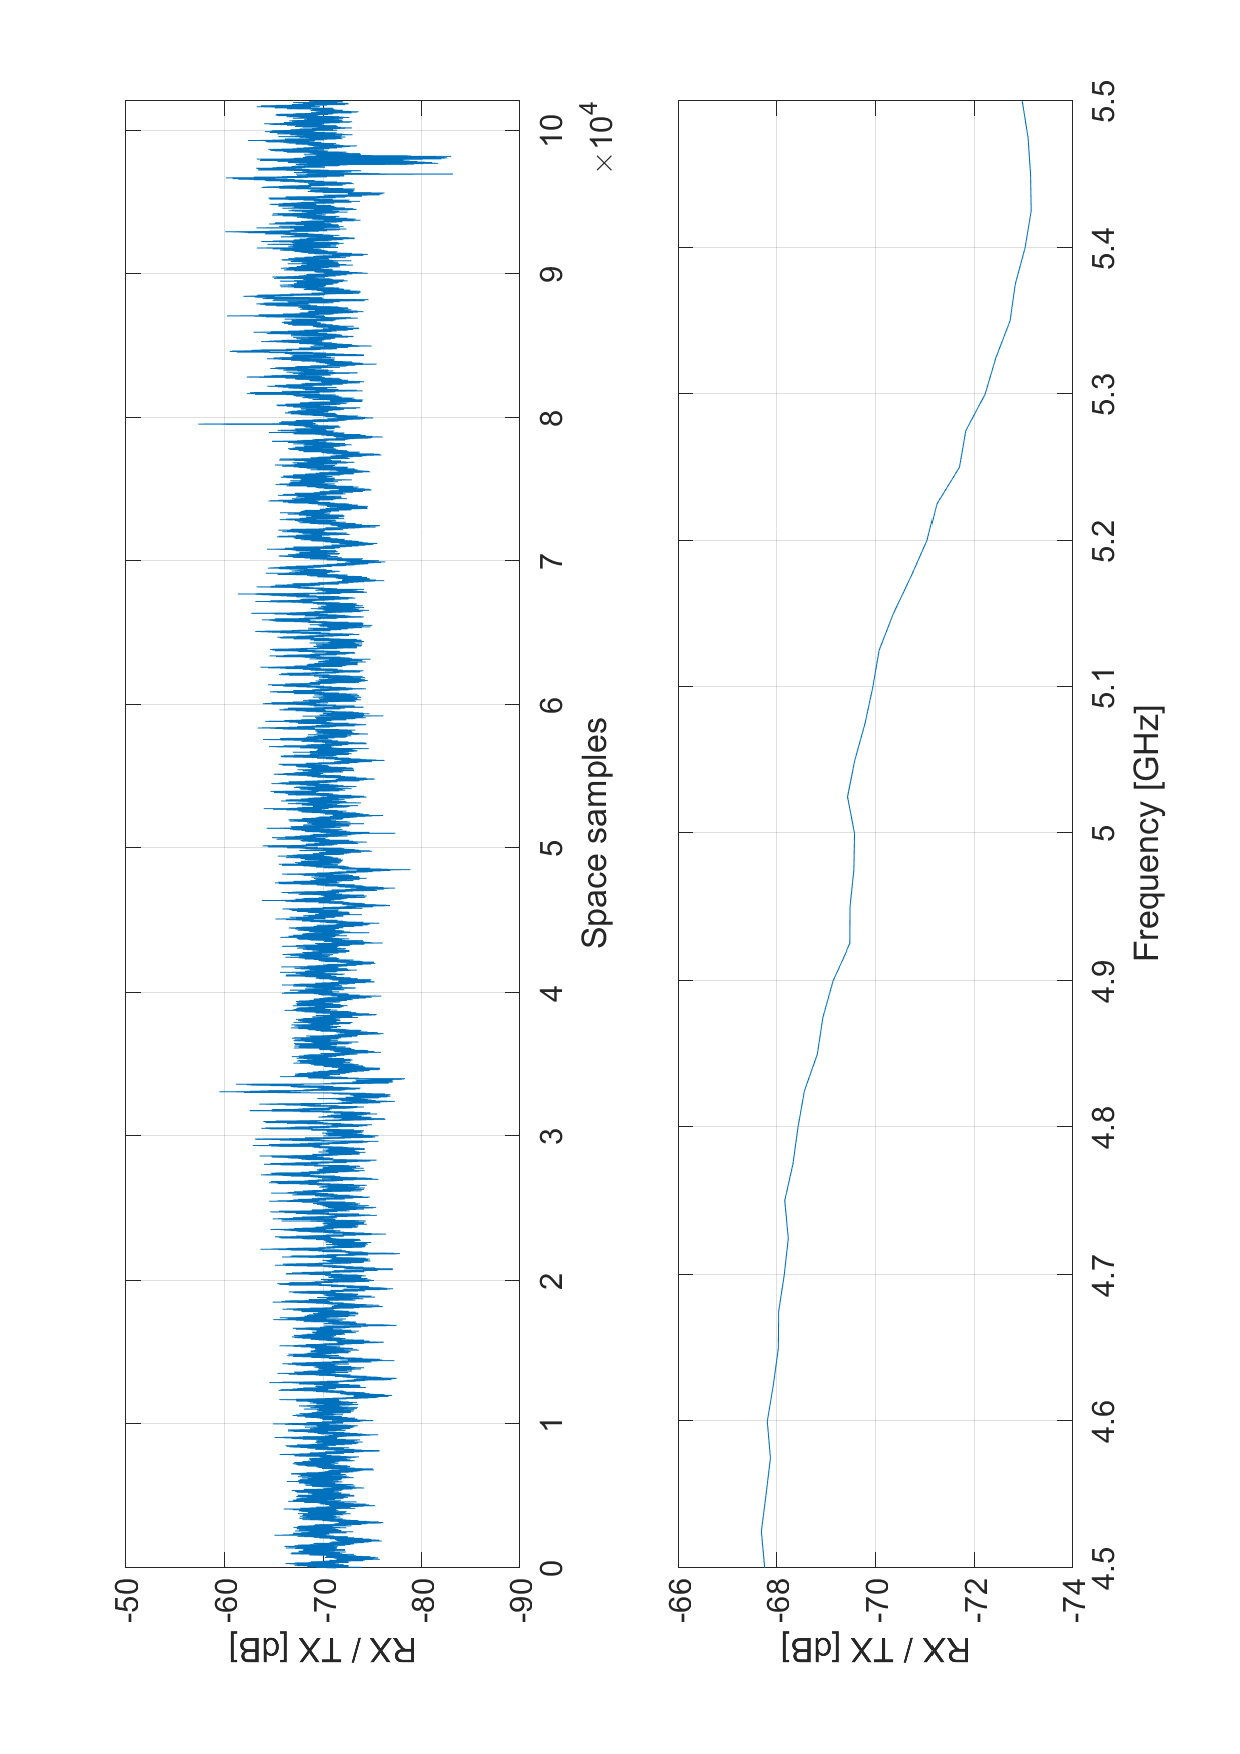
\includegraphics[height = \textwidth, angle = -90]{figures/meanFading.pdf}
% This file was created by matlab2tikz.
%
%The latest updates can be retrieved from
%  http://www.mathworks.com/matlabcentral/fileexchange/22022-matlab2tikz-matlab2tikz
%where you can also make suggestions and rate matlab2tikz.
%
\definecolor{mycolor1}{rgb}{0.00000,0.44700,0.74100}%
%
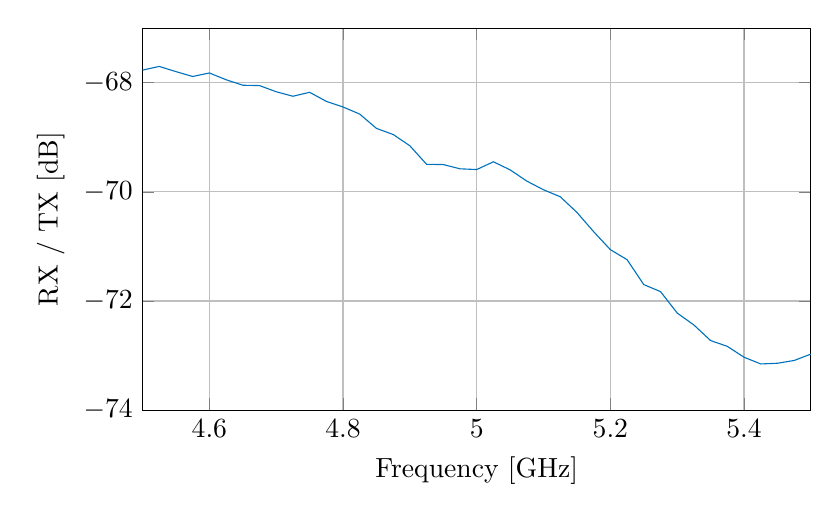
\begin{tikzpicture}

\begin{axis}[%
width=0.7\textwidth,
height=0.4\textwidth,
at={(0.758in,0.481in)},
scale only axis,
xmin=4.5,
xmax=5.5,
xlabel={Frequency [GHz]},
xmajorgrids,
ymin=-74,
ymax=-67,
ylabel={RX / TX [dB]},
ymajorgrids,
axis background/.style={fill=white}
]
\addplot [color=mycolor1,solid,forget plot]
  table[row sep=crcr]{%
4.5	-67.7676892980713\\
4.525	-67.7004021954752\\
4.55	-67.7955301958539\\
4.575	-67.8845412993962\\
4.6	-67.8205218880063\\
4.625	-67.9439627079413\\
4.65	-68.04512612016\\
4.675	-68.051565781706\\
4.7	-68.1644910960917\\
4.725	-68.2469599638715\\
4.75	-68.1744447064323\\
4.775	-68.3408515759533\\
4.8	-68.4431912057773\\
4.825	-68.5744291919179\\
4.85	-68.8363636692087\\
4.875	-68.9480881021396\\
4.9	-69.1549059751271\\
4.925	-69.4947511904151\\
4.95	-69.4993310363175\\
4.975	-69.5769572316811\\
5	-69.5906628312393\\
5.025	-69.4483437709345\\
5.05	-69.5961078771687\\
5.075	-69.8026690275714\\
5.1	-69.9616513128938\\
5.125	-70.0889574328478\\
5.15	-70.3770813009446\\
5.175	-70.7298661505624\\
5.2	-71.0591359058608\\
5.225	-71.2429090613138\\
5.25	-71.6994261918864\\
5.275	-71.8280447931612\\
5.3	-72.2209086728416\\
5.325	-72.4401711956896\\
5.35	-72.7258613771483\\
5.375	-72.8313187431047\\
5.4	-73.0312002594864\\
5.425	-73.154105653938\\
5.45	-73.1413033949649\\
5.475	-73.0904973481192\\
5.5	-72.9729692416908\\
};
\end{axis}
\end{tikzpicture}%
\caption{Average values across the frequency as per \autoref{eq:freqMean}, with values converted from linear scale to dB.}
\label{fig:meanFading}
\end{figure}

It can be seen that there is a drop of around 4 dB across the frequency, this drop can be explained by 2 factors first the antenna gain varies with around 2 dB across the frequency span \appref{ant_adix}, the other part is the \gls{PL} is dependent on frequency, by comparing PL of a free space path loss model, it can be seen that there is a drop of 1.75 dB going from 4.5 GHz to 5.5 GHz. Those two factors together can explain the drop in mean power across the span. As this can be explained the data is adjusted as:

\begin{equation}
data2 =  data \oslash \left(freqData\cdot ones(1,M,K)\right)
\end{equation}

\textbf{Spatial domain}

Likewise as the frequency domain the average is taken across the other domains, here it is assumed that the antennas even though spaced is a separate and stationary domain due to their closeness. The average is found based on the frequency corrected data as:

\begin{equation}\label{eq:spaceMean}
spaceData(k) = \frac{1}{N\cdot M}\sum_{n = 1}^{N}\sum_{m = 1}^{M} data2_{(n,m,k)}
\end{equation}

To visualize the data is restructured such that it matches the area it has been taken in see \autoref{Environment}. The data was collected by walking forth and back in the room with approx. 42 sweeps per meter or 210 sweeps per stretch. As every second stretch was walking back it has to be reversed to visualize the samples side by side. 


\begin{minipage}{0.9\textwidth}

\begin{figure}[H]
\captionsetup{belowskip=0em}
\begin{subfigure}[b]{0.326\textwidth}
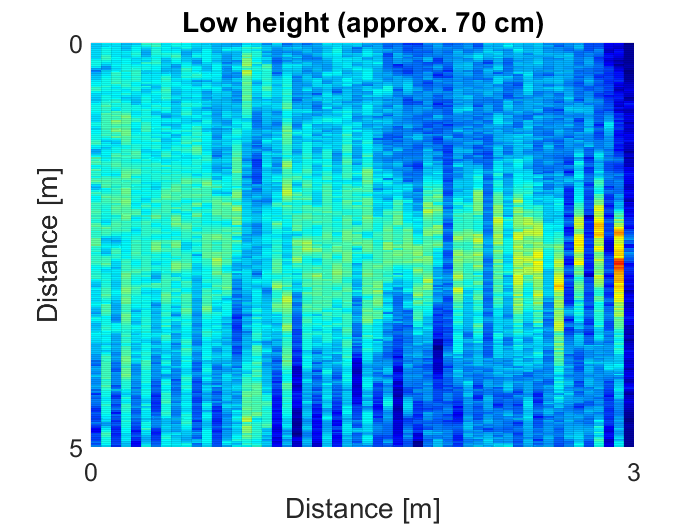
\includegraphics[width=\textwidth]{figures/Not_Norm_space_1.png}
\caption{Hallos}
\label{1}
\end{subfigure}
\begin{subfigure}[b]{0.326\textwidth}
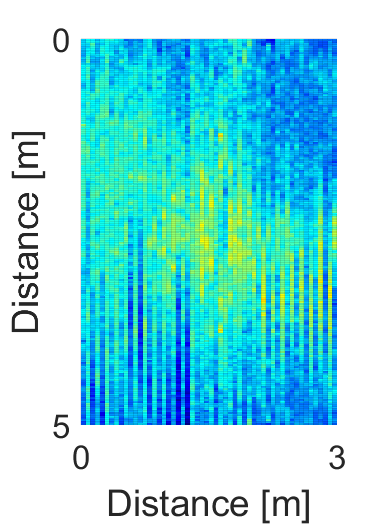
\includegraphics[width=\textwidth]{figures/Not_Norm_space_2.png}
\caption{Hallos}
\label{2}
\end{subfigure}
\begin{subfigure}[b]{0.326\textwidth}
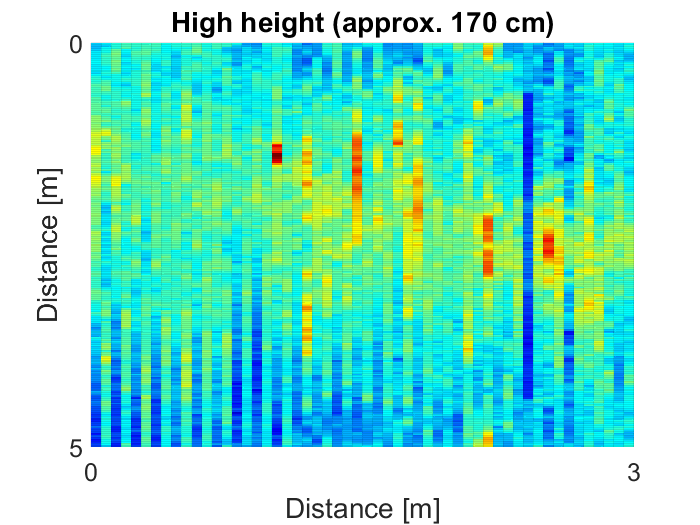
\includegraphics[width=\textwidth]{figures/Not_Norm_space_3.png}
\caption{Hallos}
\label{3}
\end{subfigure}
\captionsetup{belowskip=-1.5em}
\caption{Hallos}
\label{3}
\end{figure}
\end{minipage}%
\begin{minipage}{0.1\textwidth}
\begin{figure}[H]
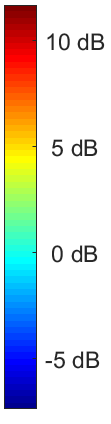
\includegraphics[width=\textwidth]{figures/Not_Norm_space_colorbar.png}
\end{figure}
\end{minipage}


%Note the reason for the spuriousness in the spatial domain has to do with the average being taken only over the 41 frequency samples at each position, where the the more smooth line in the frequency domain is an average across 102.060 samples in space. It can however be seen directly that the power level seems more or less constant across all spatial points, where it drops with frequency. This is expected as the \gls{PL} is dependent on the wavelength.  

%A condition that has to be met is that no dominant componet is present, to check this all samples are normalized with regards to the mean values seen in \autoref{fig:meanFading}, the normalize data is then fitted to a Rician distribution and the non-centrality parameter is found using matlabs \textit{fitdist} function as can be seen in \autoref{lst:a_value}. 

%\lstset{caption={Code implementation of the a value calculation.}, label=lst:a_value}
%\begin{lstlisting}
%% The measured values is stored in data which is a 41x102060 matrix with
%% the rows being frequency samples and the coloums being space samples
%
%PL = repmat(mean(data,2),1,102060);   % Determine PL by averaging across space dimension 
%dataN = data./PL;                     % Normalize data wrt. frequency
%dataS = reshape(dataN,41*102060,1);   % Reshape to vector format
%
%pd = fitdist(dataS,'Rician');         % Fit data to a Rician distribution
%pd.s                                  % Show non-centrality parameter for space domain
%
%PL = repmat(mean(data,1),41,1);       % Determine PL by averaging across frequency dimension
%dataN = data./PL;                     % Normalize data wrt. space
%dataF = reshape(dataN,41*102060,1);   % Reshape to vector format
%
%pd = fitdist(dataF,'Rician');         % Fit data to a Rician distribution
%pd.s                                  % Show non-centrality parameter for frequency domain
%\end{lstlisting}

%From this it can be found that the non-centrality parameter of the two domains are 0.0267 and 0.0319 for space and frequency domain respectively. That means that any dominant component is negligible compared to the random components, and it can therefore by concluded that the channel behaves stationary.

%\begin{figure}
%\input{figures/Norm_sapce_3.tex}
%\end{figure}
%\begin{figure}
%\input{figures/Not_Norm_sapce.tex}
%\end{figure}